The process for bootstrap calibrating the WWLLN stations and how the energy is calculated is described in \citet{Hutchins2012}.
This section walks through the code used in the processing along with the decisions behind various checks and adjustments made in the processing.

\section{Code Summary}

There are XXX main sections to the bootstrap processing:

\begin{itemize}
	\item{Process R-files into AP-files}
	\item{Calculate LWPC attenuation coefficients for each stroke-station pair}
	\item{Bootstrap calibrate the network}
	\item{Calculate stroke energy using LWPC and calibration}
	\item{Iterative re-calibrate the network}
	\item{Final energy calculation}
	\item{Run Relative Detection Efficiency Model (Chaper~\ref{ch:de})}
	\item{Move files to storage locations}
\end{itemize}

This processing requires several files, locations given relative to mlhutch@flash5.ess.washington.edu.

\begin{itemize}
	\item{\textbf{$\sim$/Process/relocate-B31Jan2013.x86-64} -- James Brundell's relocate program used to process R-files into AP-files, this version compiled for Linux 64-bit systems}
	\item{\textbf{stations.dat} -- list of current WWLLN stations, copied over from flash4 at the start every processing run.}
	\item{\textbf{lwpcv21} -- directory containing a working compiled version of the LWPC code.
		Used in generating new lookup tables as stations are added, a parallelized matlab implemtation is discussed below.}
	\item{\textbf{$\sim$/matlab/Bootstrap/} -- directory containing the necessary matlab files, available as a git directory (see Appendix~\ref{app:code}).}
	\item{\textbf{$\sim$/matlab/functions/} -- directory of necessary matlab functions used by the Bootstrap code files, also available as a git directory (see Appendix~\ref{app:code}).}
\end{itemize}

\section{LWPC}

The Long Wave Propagation Capability code is a codebase developed by \citet{Ferguson1998} that is used to calculated the electric field at a given location for a VLF transmitter at another location.
For the WWLLN energy processing it is used to estimate the attenuation between a stroke (treated as a transmitter) and a station.
The original LWPC code has been altered in two ways: first the Windows-compiler specific code has been replaced with GCC compilable code, second all warning have been removed to produce output of a constant shape (for reading into MATLAB).
All edits in the source code have been marked by my initials of MH.

\subsection{Compiling}

To recompile LWPC two bash scripts need to be run.
The first is \textbf{BuildData.cmd}, BuildData recompiles the data files that contain the surface parameters such as ground conductivity and coastlines.
The second step is to run \textbf{buildlwpc.cmd}, this should compile the program and result in an executable called LWPC.
To test a successful compile run the script \textbf{run\_bench.cmd}, if it runs successfully it is compiled, if not consult the \textbf{Readme - Unix.txt} file that has some common troubleshooting steps.

The last step in setting up LWPC is to set the \textbf{lwpcDAT.loc} file to point towards the \textbf{data} folder.

\subsection{Running}

LWPC is run from the command line with the structure:

\begin{verbatim}
./LWPC test1.inp
\end{verbatim}

Where \textbf{test1.inp} is formatted as per the structure in \textbf{User\_manual.pdf}.
The matlab implemtations discussed below automatically generate formatted input files.

The result of running LWPC is an output file the specifies the electric field at various distance along the path from the transmitter to receiver.
It is also capable of outputting plots, azimuthal dependence, and many other features not utilized in this research.

\subsection{Matlab Function}

A matlab implementation of LWPC is available as a git repository (see Appendix~\ref{app:code}).
This implantation allows for LWPC to called in matlab with:

\begin{verbatim}
LWPCpar(freq,lat,long,time,stat_lat,stat_long,model)
\end{verbatim}

Where freq is the transmitter frequency, lat/long is the transmitter location, time is the date and time, stat\_lat/stat\_long are the receiver locations, and model is the ionospheric model used.
If model is set to ``time'' then day and night is considered in the calculation, if it is set to ``day'' or ``night'' an all day or all night ionosphere will be used.

LWPCpar as the advantage of being runnable within matlab parallelized loops (parfor).
While LWPC itself cannot be run in parallel, this method simply copies the LWPC directory to allow each matlab instance it's own copy.

\section{Lookup Tables}

While LWPC can be parallelized it is still too slow to run faster than realtime for WWLLN processing.
As a result two sets of lookup tables are generated for each station with the pre-calculated LWPC electric field values.

The lookup tables are part of the main Bootstrap directory under the names \textbf{lookup\_day.dat} and \textbf{lookup\_night.dat}.
Each of these files are tab-delimited text with the format given in Table~\ref{app:table:lookup}.
The tables list the electric field measured the the station given a 100~kW transmitter in each grid point on the globe.
The latest lookup tables are at a resolution of $2^\circ$.

\begin{table}[h!]
\begin{center}
\begin{tabular}{|p{1.5in}|p{1.75in}|p{1.75in}|p{1in}|}
\hline
\rule{0pt}{3ex}
Station Name	&Station North Latitude	&	Station East Longitude & \\ 
\hline
\rule{0pt}{3ex}
E-field at (-179,89)	& E-field at (-177,89) &	E-field at (-175,89) & \dots \\ 
\hline
\rule{0pt}{3ex}
E-field at (-179,87)	& E-field at (-177,87) &	E-field at (-175,87) & \dots \\ 
\hline
\rule{0pt}{3ex}
E-field at (-179,85)	& E-field at (-177,85) &	E-field at (-175,85) & \dots \\ 
\hline
\rule{0pt}{3ex}
\dots	& \dots &	\dots & \dots \\ 
\hline
\end{tabular}
\end{center}
\caption{Format for \textbf{lookup\_day.dat} and \textbf{lookup\_night.dat} data files for a resolution of $2^\circ$.}
\label{app:table:lookup}
\end{table}

An example of a lookup table for the all day ionosphere for Dunedin station is shown in Figure~\ref{app:fig:lookup}.

\begin{figure}[ht!]
   \centering
   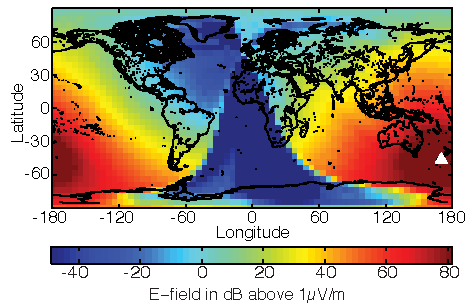
\includegraphics[scale=1]{Energy/Figures/PPS_Lookup.pdf} 
   \caption{Lookup table for an all day ionosphere for Dunedin station.}
   \label{app:fig:lookup}
\end{figure}

\subsection{Generation}

The LWPC lookup tables are generated automatically with the matlab script \textbf{$\sim$/Bootstrap/Lookup_automation.m} that is called at the start of the daily energy processing.
The script checks the current number of stations in the \textbf{.dat} files and compares it to the most recent \textbf{stations.dat} file.
If there are a new entries in the \textbf{stations.dat} then the script proceeds to make the lookup tables.

The automatic script calculates the electric field at every grid point for 11 frequencies ranging from 8~kHz to 18~kHz, and averages them together to add to the \textbf{.dat} files.

The same script can be run for specific stations with the \textbf{$\sim$/matlab/lwpcpar/lwpc\_generate.m} script.

Tables generated with either script can be validated with the \textbf{$\sim$/matlab/Bootstrap/lookup\_validation.m} scipt.
This script checks each grid point to ensure there is a real number there, sometimes LWPC generates errors for very specific locations.
If there is no valid electric field value at that spot it is reprocessed by offsetting the transmitter by a fraction of a degree.

\subsection{Code}

\section{Bootstrap and Calibration Process}

\section{Matlab Code}

\subsection{Rerunning Lost Days}

\subsection{Automation}

\subsection{Time Estimates}

\section{Relative Detection Efficiency Code}

\subsection{Point to Paper}

\subsection{Code Summary}

\subsection{Code Description and Location}

\subsection{Output Interpretation}

\subsection{Matlab Code}